\documentclass[tikz]{standalone}
\usepackage[utf8x]{inputenc}
\usepackage{tikz}
\usepackage{circuitikz}
\usetikzlibrary{arrows, patterns, shapes, decorations.markings, decorations.pathmorphing}
\begin{document}
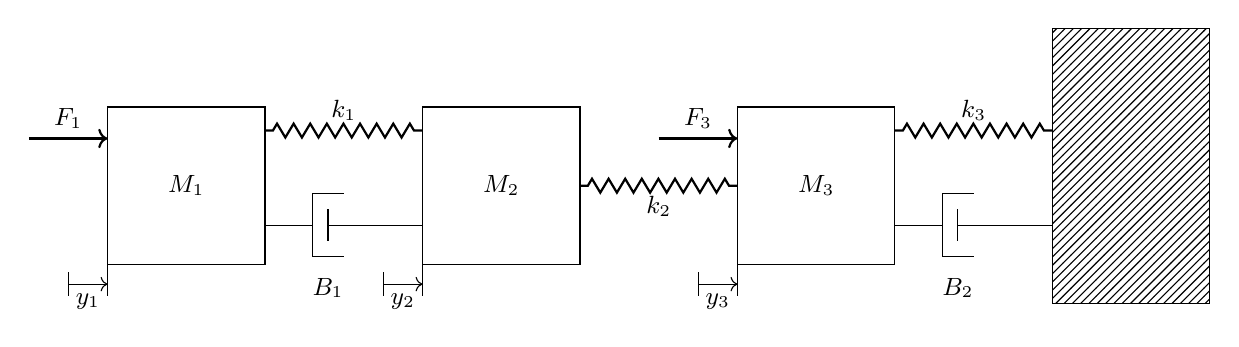
\begin{tikzpicture}[font=\small]
    \tikzstyle{spring}=[thick,decorate,decoration={zigzag,pre length=0.1cm,post
  length=0.1cm,segment length=6}]
    \draw [->,thick] (-1,1.6) -- node [above, midway] {$F_{1}$}(0,1.6);
    \draw (0,-0.4) -- (0,0);
    \draw (-0.5,-0.1) -- (-0.5,-0.4);
    \draw [->](-0.5,-0.25) -- node [midway, below] {$y_{1}$}(0,-0.25);
    \draw (0,0) rectangle node {$M_{1}$}(2,2);
    \draw[spring] (2,1.7) -- node [above] {$k_{1}$} (4,1.7);
    \draw (2,0.5) -- (2.6,0.5);
    \draw (2.6,0.1) -- (2.6,0.9);
    \draw (2.6,0.1) -- (3,0.1);
    \draw (2.8,-0.3) node {$B_{1}$};
    \draw (2.6,0.9) -- (3.0,0.9);
    \draw (2.8,0.3) -- (2.8,0.7);
    \draw (2.8,0.5) -- (4,0.5);
    \draw (4,-0.4) -- (4,0);
    \draw (3.5,-0.1) -- (3.5,-0.4);
    \draw [->](3.5,-0.25) -- node [midway, below] {$y_{2}$}(4,-0.25);
    \draw (4,0) rectangle node {$M_{2}$}(6,2);
    \draw [spring] (6,1) -- node [below] {$k_{2}$} (8,1);
    \draw [->,thick] (7,1.6) -- node [above, midway] {$F_{3}$}(8,1.6);
    \draw (8,-0.4) -- (8,0);
    \draw (7.5,-0.1) -- (7.5,-0.4);
    \draw [->](7.5,-0.25) -- node [midway, below] {$y_{3}$}(8,-0.25);
    \draw (8,0) rectangle node {$M_{3}$} (10,2);
    \draw[spring] (10,1.7) -- node [above] {$k_{3}$} (12,1.7);
    \draw (10,0.5) -- (10.6,0.5);
    \draw (10.6,0.1) -- (10.6,0.9);
    \draw (10.6,0.1) -- (11,0.1);
    \draw (10.8,-0.3) node {$B_{2}$};
    \draw (10.6,0.9) -- (11.0,0.9);
    \draw (10.8,0.3) -- (10.8,0.7);
    \draw (10.8,0.5) -- (12,0.5);
    \draw [pattern=north east lines] (12,-0.5) rectangle (14,3);
\end{tikzpicture}
\end{document}